\documentclass[10pt]{article}
\usepackage[margin=0.85in]{geometry}
\usepackage{graphicx,booktabs,longtable,float,xcolor}
\setlength{\parskip}{0.4em}\setlength{\parindent}{0pt}
\title{RNGD Hotel Schematic: Final Report\\\large 2D plans, 3D views, interiors, program and code screen}
\author{RNGD semester proof of concept --- prototype, not for construction}
\date{\today}
\begin{document}
\maketitle
\tableofcontents

\section{Summary}
The program has 117 guest keys in 21 rows totalling 59,350 SF net. The source gross
area is 74,195 SF. Using the kickoff-meeting factors (33\% circulation, 8\% wall burden), required gross
is 85,300 SF. The schematic places all keys across five upper levels of double-loaded corridor.
Two IBC screens from RNGD's rule set fail: the number of stories above grade and the dead-end corridor length.

\section{Program and gross area}
Source: Project Renegade Living + Lodging Prototype, cover sheet (06/20/25). Guest-room areas are type averages. Source gross by level: Level 1 12,485, Level 2 12,342, Level 3 12,342, Level 4 12,342, Level 5 12,342, Level 6 12,342.
\begin{longtable}{p{7.4cm}rrl}\toprule Room type & Count & Area (SF) & Category \\ \midrule
ADA Corner Suite & 1 & 852 & guest \\
ADA King Spa & 2 & 920 & guest \\
ADA QQ & 2 & 892 & guest \\
ADA Suite & 2 & 1,278 & guest \\
Corner Suite & 2 & 1,728 & guest \\
King & 69 & 23,692 & guest \\
King Spa & 3 & 1,379 & guest \\
QQ & 33 & 11,342 & guest \\
Suite & 3 & 1,920 & guest \\
Corridor & 1 & 1,335 & shared \\
Gym & 1 & 968 & shared \\
Lobby & 1 & 2,865 & shared \\
Restrooms (M/W) & 1 & 405 & shared \\
Luggage & 1 & 122 & shared \\
BOH / Bus & 1 & 1,718 & boh \\
Hotel Kitchen / Pantry & 1 & 331 & boh \\
BOH storage (BOH, Housekeeping, Janitor, Ice, IT, Supplies) & 1 & 1,611 & boh \\
Loading & 1 & 282 & boh \\
MEP Service & 1 & 309 & boh \\
Stairs & 1 & 1,868 & core \\
White Box Retail (tenant) & 1 & 3,533 & tenant \\
\bottomrule\end{longtable}

\section{Ground level and site}
\begin{figure}[H]\centering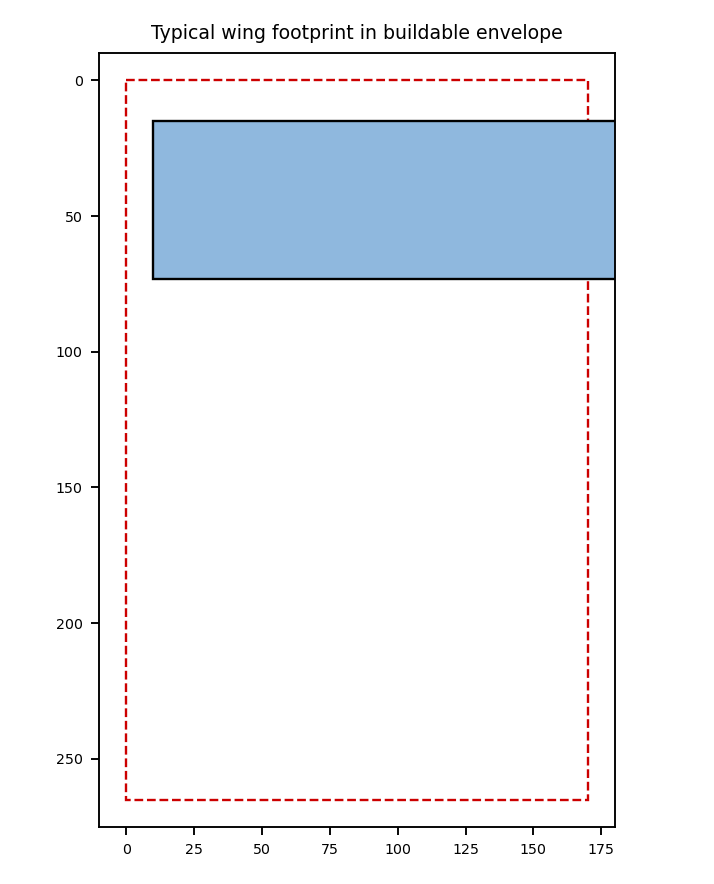
\includegraphics[width=0.42\linewidth]{png/site_envelope.png}\caption{Typical wing footprint in the buildable envelope (synthetic lot, 170 x 265 ft).}\end{figure}
\begin{figure}[H]\centering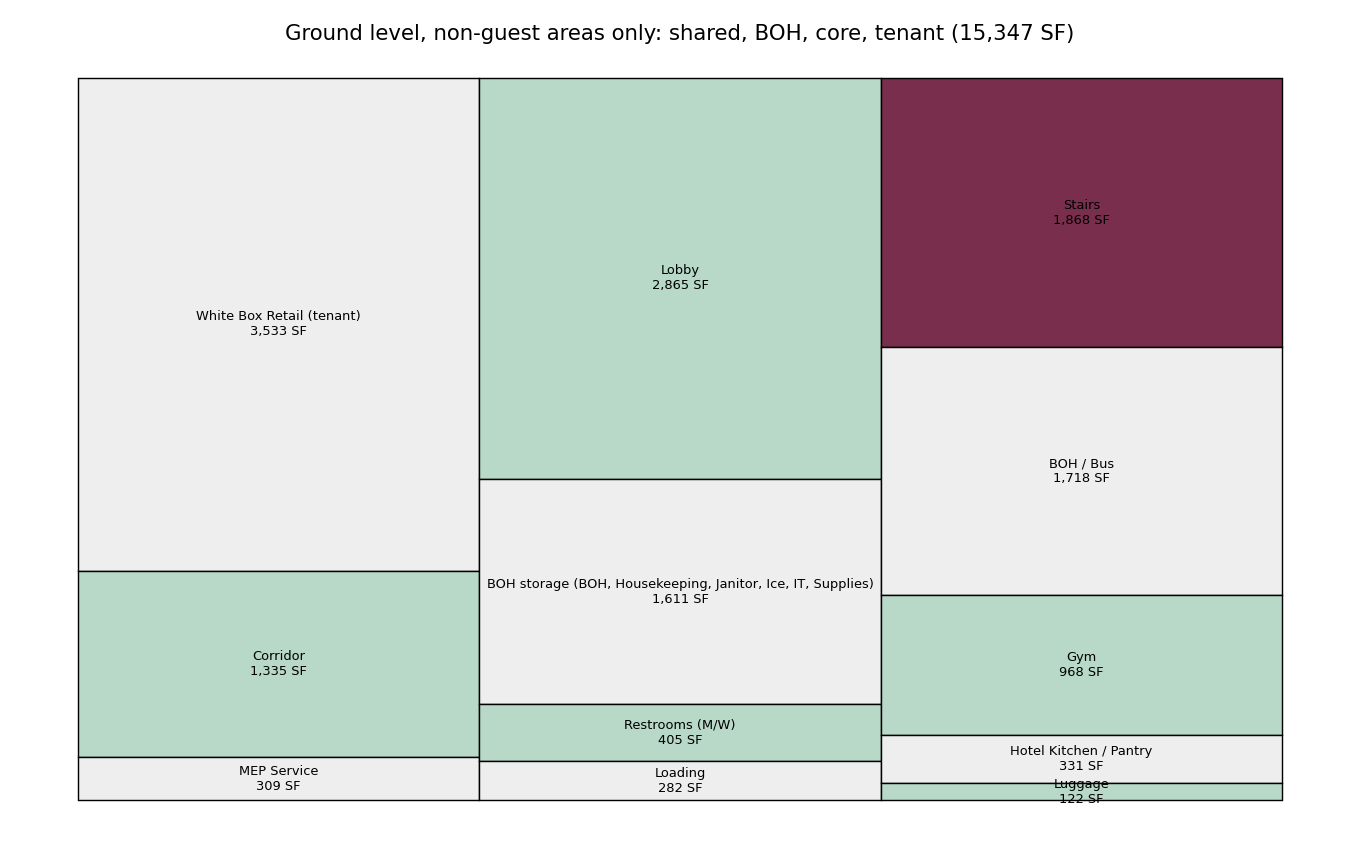
\includegraphics[width=0.95\linewidth]{png/ground_blocks.png}\caption{Ground level, non-guest areas only, as a block diagram from program areas. Not a measured plan.}\end{figure}

\section{2D plans}
\begin{figure}[H]\centering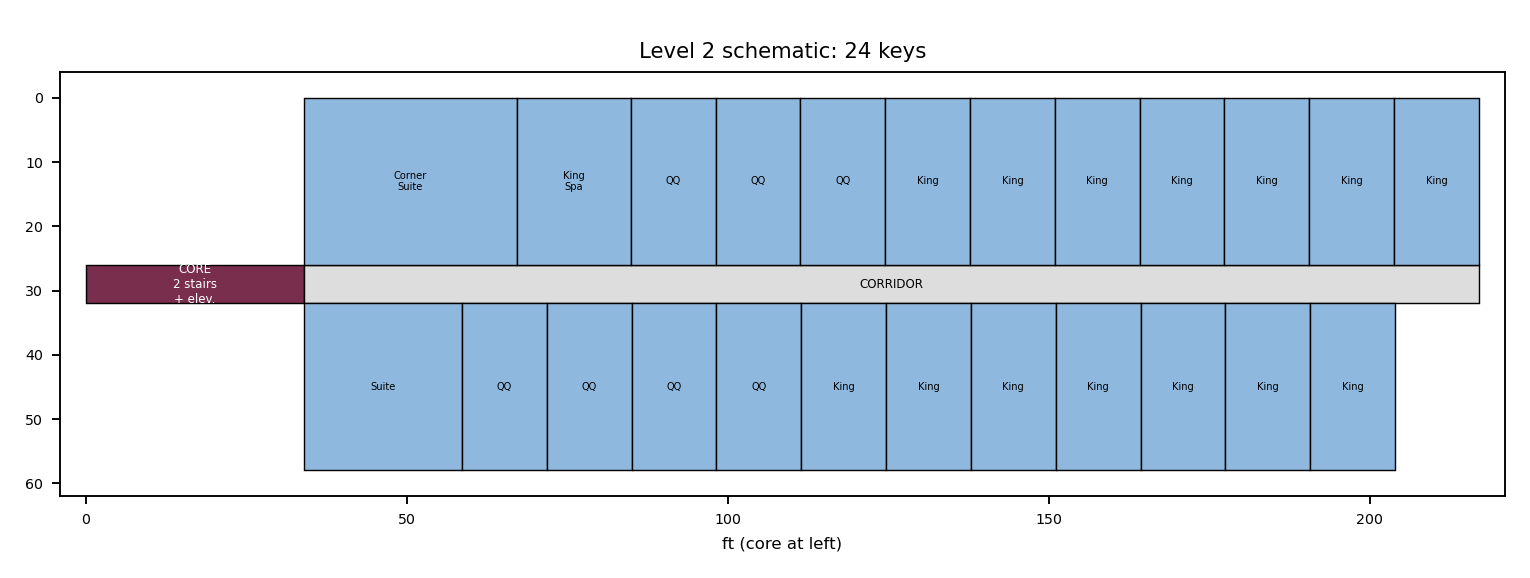
\includegraphics[width=\linewidth]{png/level_2_plan.png}\caption{Level 2 plan: 24 guest keys.}\end{figure}
\begin{figure}[H]\centering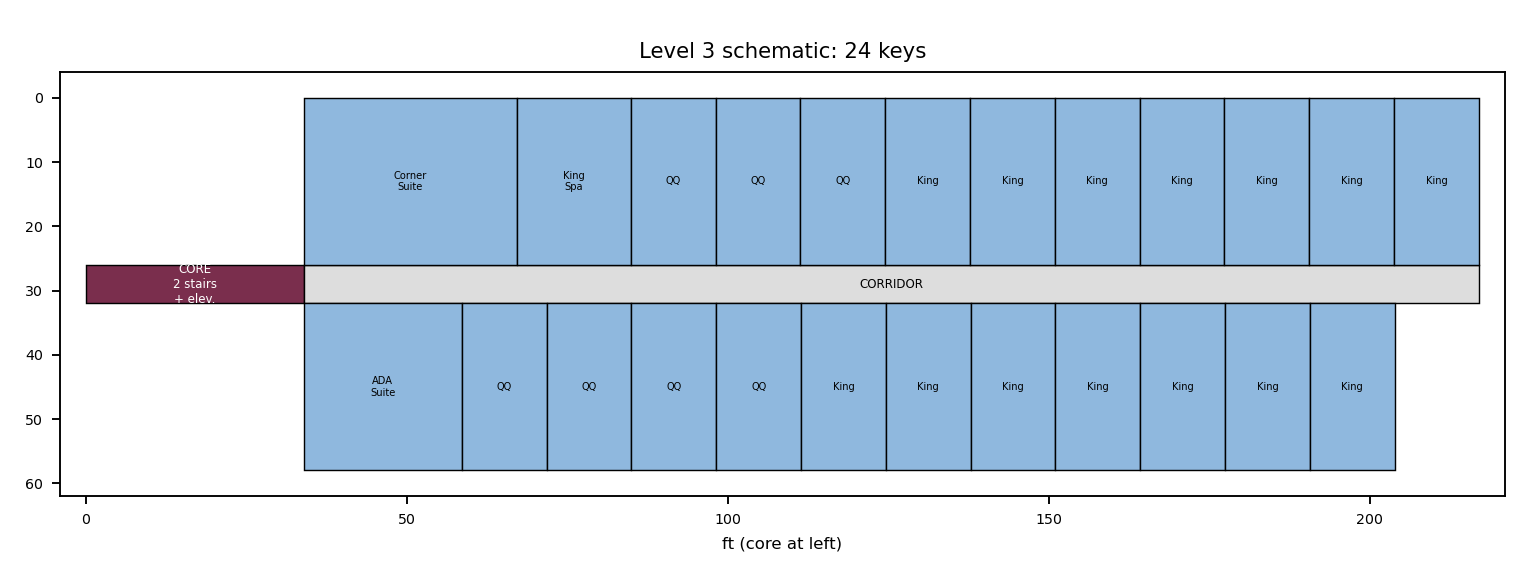
\includegraphics[width=\linewidth]{png/level_3_plan.png}\caption{Level 3 plan: 24 guest keys.}\end{figure}
\begin{figure}[H]\centering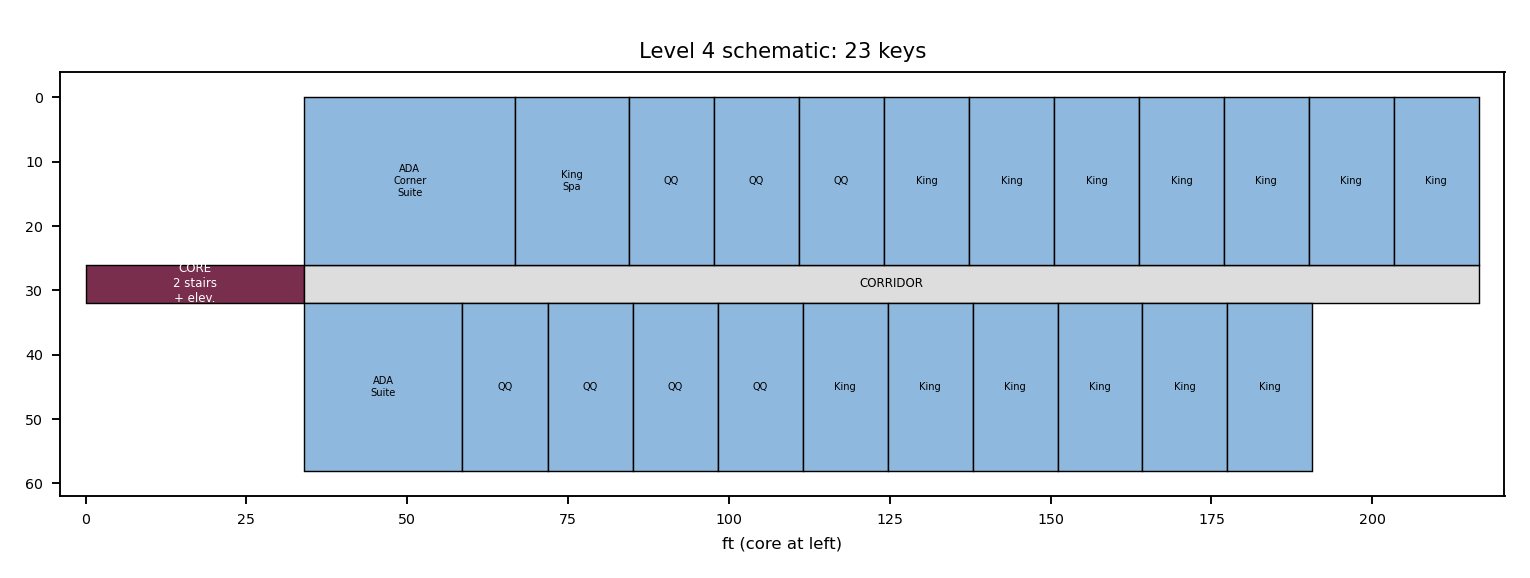
\includegraphics[width=\linewidth]{png/level_4_plan.png}\caption{Level 4 plan: 23 guest keys.}\end{figure}
\begin{figure}[H]\centering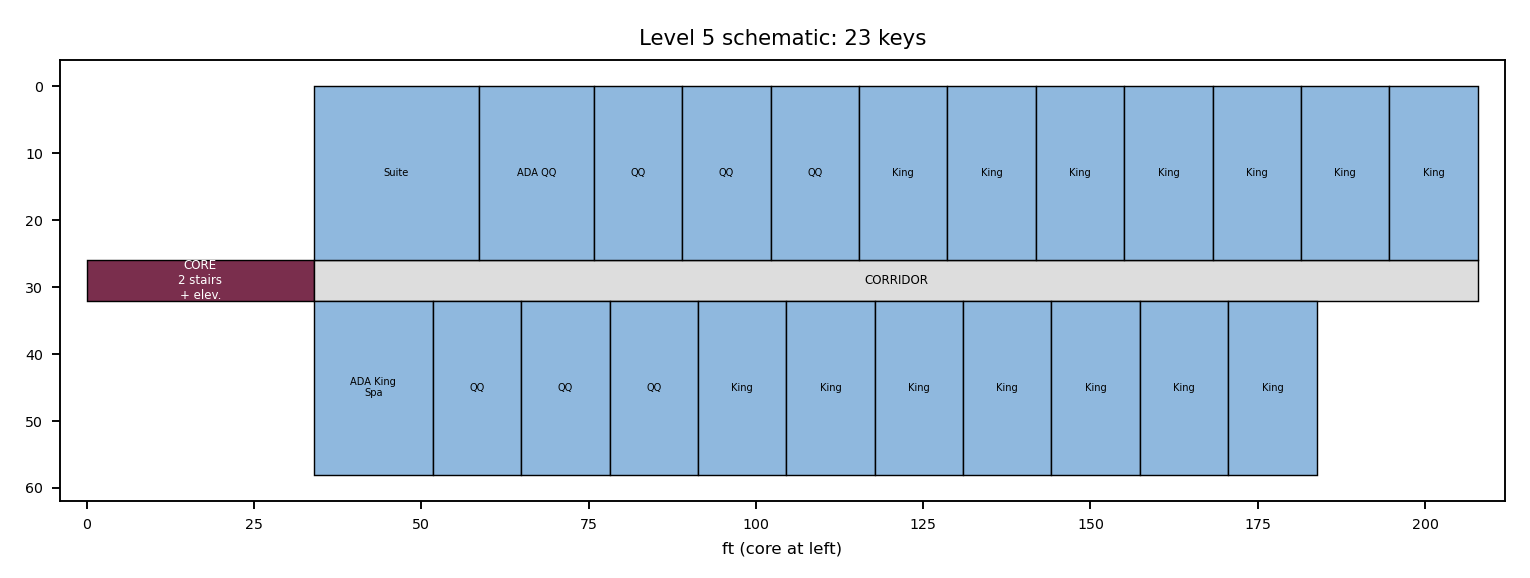
\includegraphics[width=\linewidth]{png/level_5_plan.png}\caption{Level 5 plan: 23 guest keys.}\end{figure}
\begin{figure}[H]\centering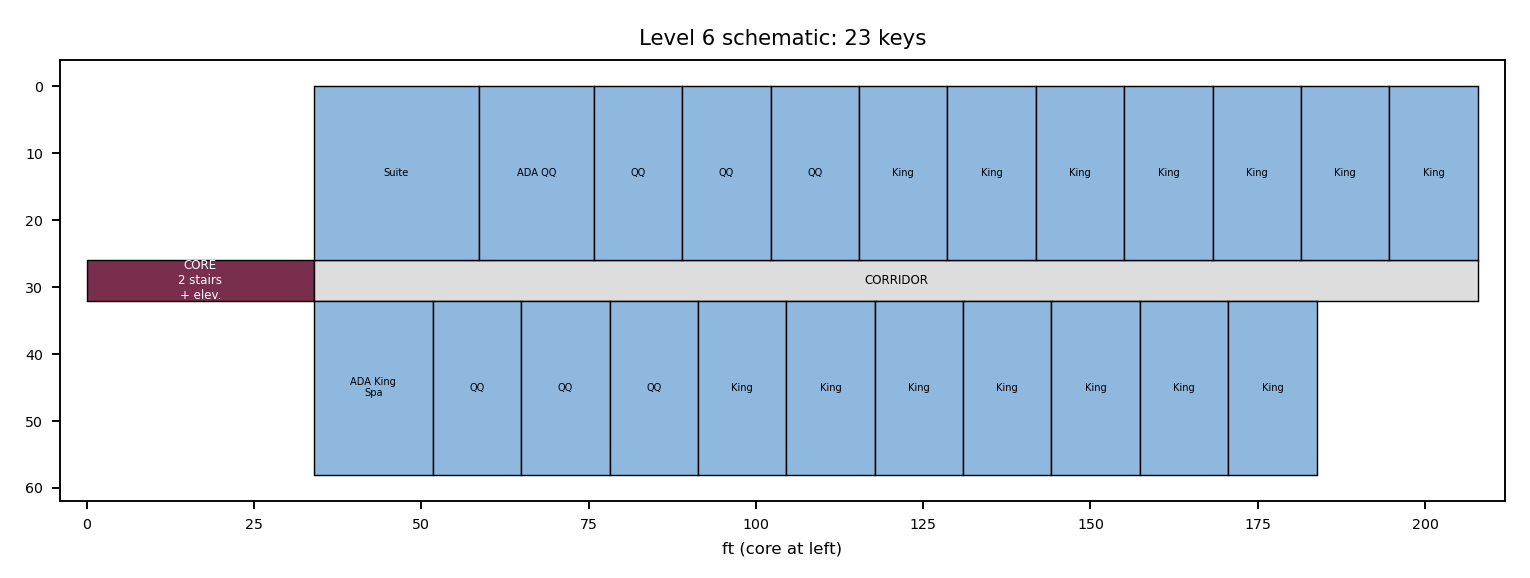
\includegraphics[width=\linewidth]{png/level_6_plan.png}\caption{Level 6 plan: 23 guest keys.}\end{figure}

\section{3D building and interior views}
The 3D views are axonometric models drawn with matplotlib. They are not OpenGL renders and have no furniture beyond the
interior sketches below.
\begin{figure}[H]\centering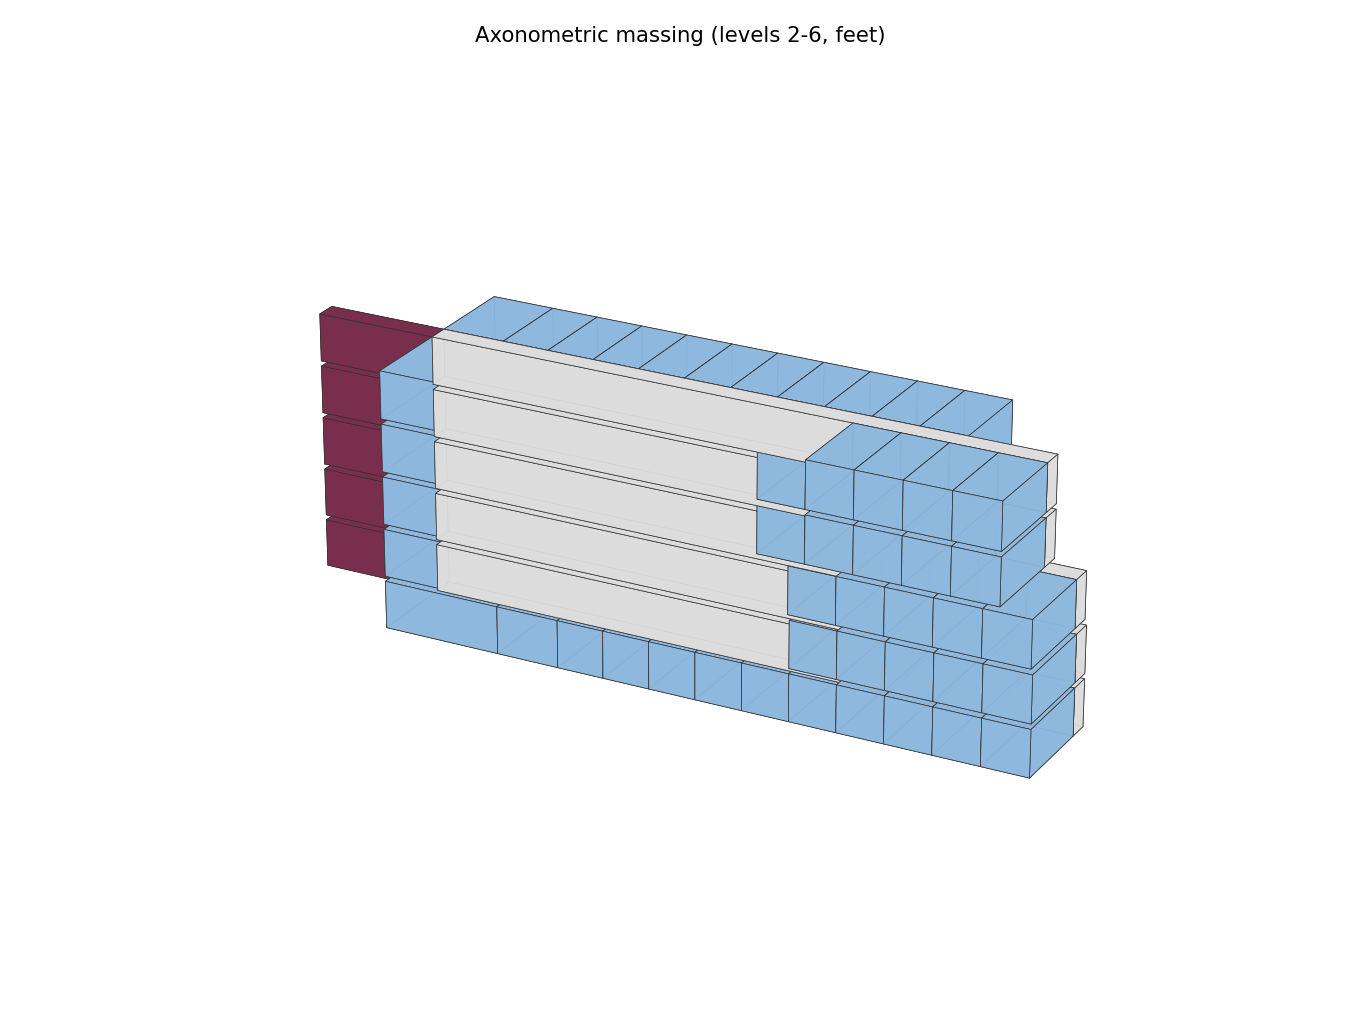
\includegraphics[width=0.85\linewidth]{png/building_3d.png}\caption{Axonometric massing of the upper levels.}\end{figure}
\begin{figure}[H]\centering
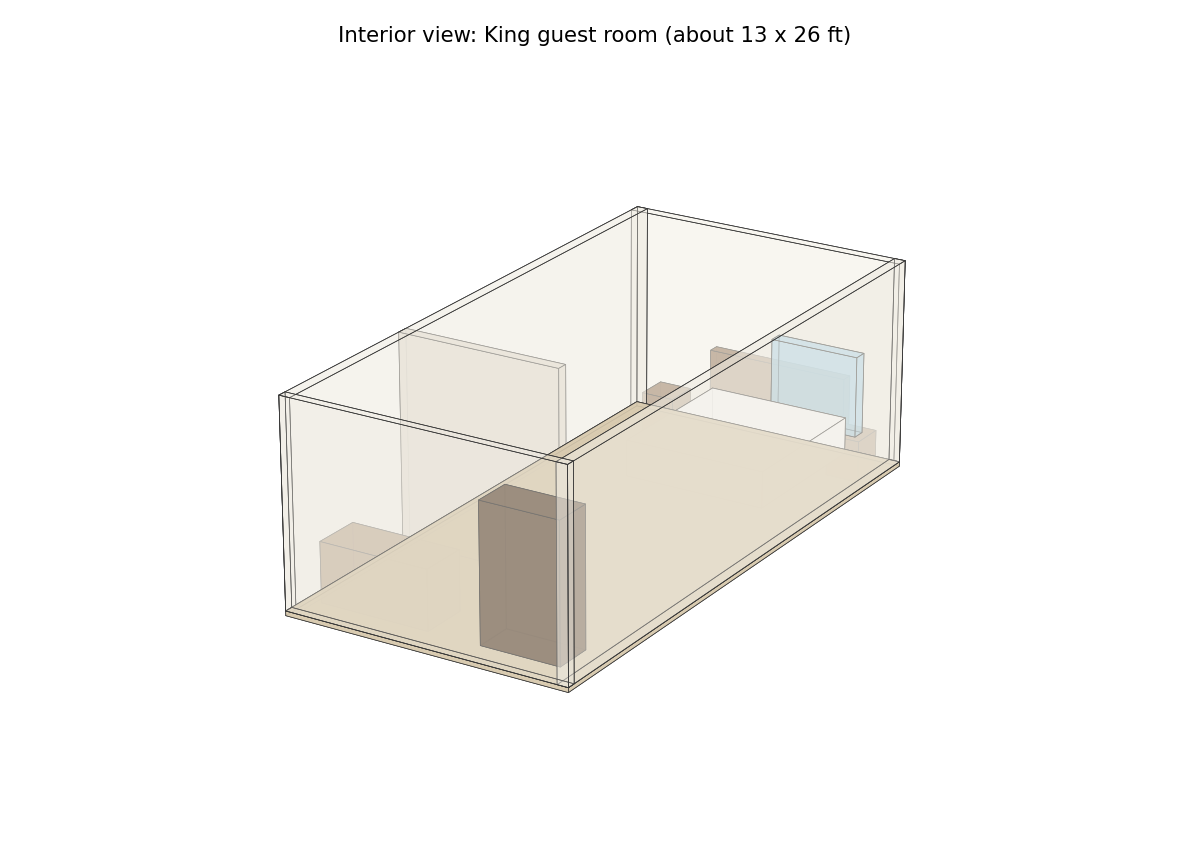
\includegraphics[width=0.48\linewidth]{png/interior_king.png}\hfill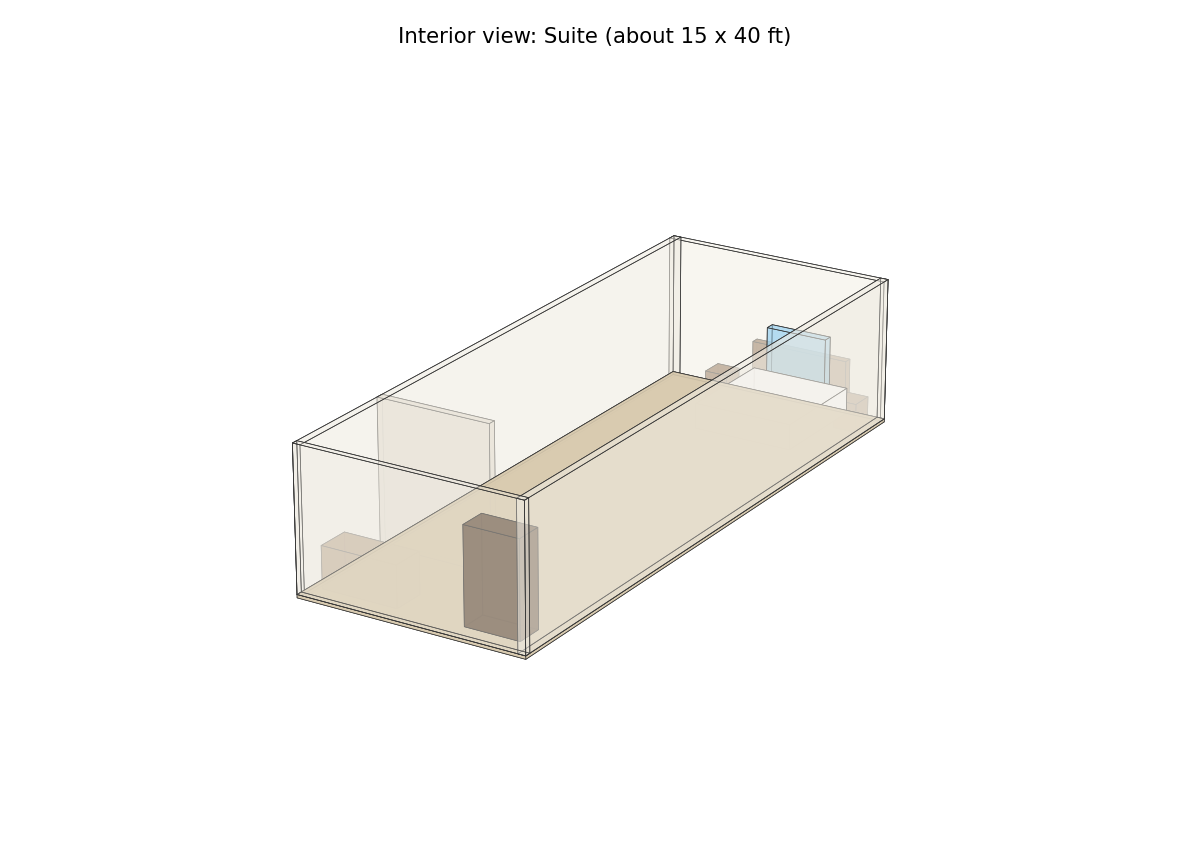
\includegraphics[width=0.48\linewidth]{png/interior_suite.png}
\caption{Interior sketches: King guest room (left) and Suite (right). Dimensions are typical, not from a drawing.}\end{figure}

\section{Code and program screen}
Checks use RNGD's 2021 IBC rule set (CSV). The screen is planning-level, not a code determination.
\begin{longtable}{p{4.4cm}p{5cm}p{3.2cm}l}\toprule Check & Required & Provided & Status \\ \midrule
Keys placed & 117 & 117 & PASS \\
Stories above grade & $\le$ 5 (IBC-R1-007, Type IIA sprinklered R-1) & 6 & FAIL \\
Building height (ft) & $\le$ 85 (IBC-R1-005, Type IIA) & 66.5 & PASS \\
Dead-end corridor (ft) & $\le$ 50 (IBC-R1-027) & 183 & FAIL \\
Exit travel distance (ft) & $\le$ 250 (IBC-R1-023) & 183 & PASS \\
Fits buildable envelope & 170 x 265 ft & 217 x 58 ft & PASS \\
\bottomrule\end{longtable}

\section{IBC rule set (from RNGD CSV)}
42 rules. 8 were evaluated against this layout. The rest need space-level
occupancy modelling that this prototype does not do yet.
\begin{longtable}{p{1.6cm}p{2.6cm}p{5.2cm}p{1.1cm}p{1.6cm}p{1.3cm}p{1.3cm}p{1.5cm}}
\toprule
rule\_id & category & rule\_name & operator & value & units & hard\_soft & evaluated\_here \\ \midrule \endhead
IBC-R1-001 & Occupancy & R-1 transient hotel classification & eq & R-1 & classification & Hard & no \\
IBC-R1-002 & Mixed Use & Small accessory assembly space classification & < & 50 occupants or 750 sf & threshold & Hard & no \\
IBC-R1-003 & Fire Protection & Automatic sprinkler required for Group R & requires & Automatic sprinkler system & system & Hard & no \\
IBC-R1-004 & Height / Stories & Allowable height and stories depend on occupancy, construction type, and spri... & lookup & Table 504.3 / 504.4 & lookup & Hard & no \\
IBC-R1-005 & Height / Stories & R occupancy sprinklered Type IIA allowable height & $\le$ & 85 & ft & Hard & yes \\
IBC-R1-006 & Height / Stories & R occupancy sprinklered Type IIB allowable height & $\le$ & 75 & ft & Hard & yes \\
IBC-R1-007 & Height / Stories & R-1 sprinklered Type IIA allowable stories & $\le$ & 5 & stories above grade plane & Hard & yes \\
IBC-R1-008 & Height / Stories & R-1 sprinklered Type IIB allowable stories & $\le$ & 5 & stories above grade plane & Hard & yes \\
IBC-R1-010 & Area & R-1 Type IIA allowable area factor, multistory sprinklered & $\le$ & 72000 & sf per story base factor & Hard & no \\
IBC-R1-011 & Area & R-1 Type IIB allowable area factor, multistory sprinklered & $\le$ & 48000 & sf per story base factor & Hard & no \\
IBC-R1-012 & High-Rise Screen & High-rise threshold screen & > & 75 & ft to occupied floor & Hard & no \\
IBC-R1-013 & Egress & R-1 single-exit space maximum occupant load & $\le$ & 10 & occupants & Hard & no \\
IBC-R1-014 & Egress & R-1 single-exit common path maximum & $\le$ & 75 & ft & Hard & no \\
IBC-R1-015 & Egress & Minimum exits per story: 1-500 occupants & eq & 2 & exits/access to exits & Hard & yes \\
IBC-R1-016 & Egress & Minimum exits per story: 501-1000 occupants & eq & 3 & exits/access to exits & Hard & yes \\
IBC-R1-017 & Egress & Minimum exits per story: over 1000 occupants & eq & 4 & exits/access to exits & Hard & no \\
IBC-R1-018 & Egress & Exit separation in sprinklered building & $\ge$ & 1/3 of maximum overall diagonal & ratio & Hard & no \\
IBC-R1-019 & Egress & Stair minimum width & $\ge$ & 44 & in & Hard & no \\
IBC-R1-020 & Egress & Stair minimum width for occupant load under 50 & $\ge$ & 36 & in & Hard & no \\
IBC-R1-021 & Egress & Stair maximum riser height & $\le$ & 7 & in & Hard & no \\
IBC-R1-022 & Egress & Stair minimum tread depth & $\ge$ & 11 & in & Hard & no \\
IBC-R1-023 & Egress & R exit access travel distance, sprinklered & $\le$ & 250 & ft & Hard & yes \\
IBC-R1-024 & Corridors & R corridor fire-resistance rating & eq & 0.5 & hour & Hard & no \\
IBC-R1-025 & Corridors & Default minimum corridor width & $\ge$ & 44 & in & Hard & no \\
IBC-R1-026 & Corridors & Minimum corridor width when occupant load is under 50 & $\ge$ & 36 & in & Hard & no \\
IBC-R1-027 & Corridors & Dead-end corridor maximum for sprinklered R-1 & $\le$ & 50 & ft & Hard & yes \\
IBC-R1-028 & Doors & Minimum clear width of required egress door opening & $\ge$ & 32 & in clear & Hard & no \\
IBC-R1-029 & Egress & Minimum means-of-egress ceiling height & $\ge$ & 7.5 & ft & Hard & no \\
IBC-OL-001 & Occupant Load & Area-based occupant load calculation & formula & Area ÷ factor & occupants & Hard & no \\
IBC-OL-002 & Occupant Load & Assembly without fixed seats - concentrated & divide\_round\_up & 7 & sf/person net & Hard & no \\
IBC-OL-003 & Occupant Load & Assembly without fixed seats - standing & divide\_round\_up & 5 & sf/person net & Hard & no \\
IBC-OL-004 & Occupant Load & Assembly without fixed seats - unconcentrated & divide\_round\_up & 15 & sf/person net & Hard & no \\
IBC-OL-005 & Occupant Load & Business areas & divide\_round\_up & 150 & sf/person gross & Hard & no \\
IBC-OL-006 & Occupant Load & Exercise rooms & divide\_round\_up & 50 & sf/person gross & Hard & no \\
IBC-OL-007 & Occupant Load & Kitchens, commercial & divide\_round\_up & 200 & sf/person gross & Hard & no \\
IBC-OL-008 & Occupant Load & Accessory storage / mechanical equipment room & divide\_round\_up & 300 & sf/person gross & Hard & no \\
IBC-OL-009 & Occupant Load & Mercantile & divide\_round\_up & 60 & sf/person gross & Hard & no \\
IBC-OL-010 & Occupant Load & Mercantile storage / stock / shipping & divide\_round\_up & 300 & sf/person gross & Hard & no \\
IBC-OL-011 & Occupant Load & Parking garages & divide\_round\_up & 200 & sf/person gross & Hard & no \\
IBC-OL-012 & Occupant Load & Residential & divide\_round\_up & 200 & sf/person gross & Hard & no \\
IBC-OL-013 & Occupant Load & Pool / rink area & divide\_round\_up & 50 & sf/person gross & Hard & no \\
IBC-OL-014 & Occupant Load & Pool / rink decks & divide\_round\_up & 15 & sf/person gross & Hard & no \\
\bottomrule\end{longtable}

\section{Workbook data (from RNGD XLSX)}
\subsection{Workbook: Project\_Config}
\begin{longtable}{p{3cm}p{3cm}p{3cm}}
\toprule
Field & Working Value & Status / Note \\ \midrule \endhead
Base code & 2021 International Building Code & Fixed \\
Jurisdiction layer &  & Per RNGD direction; base code only \\
Project type & New construction & Fixed for prototype \\
Primary occupancy & Group R-1 transient hotel & Fixed \\
Stories & 5 stories above grade plane & Fixed for current prototype \\
Sprinkler protection & Fully sprinklered; NFPA 13 assumption & Fixed for current prototype \\
Construction type & Type II; IIA vs IIB not yet locked & Keep both applicable Chapter 5 rows until subtype is confirmed \\
High-rise strategy & Screen only & Five-story prototype should still be checked against the 75-ft occupied-floor threshold if floor-to-floor heights are unusual \\
Accessibility scope & Not yet decided & IBC Chapter 11 can be added later if the team wants it inside this base-code CSV \\
\bottomrule\end{longtable}
\subsection{Workbook: Occupant\_Load\_Factors}
\begin{longtable}{p{3cm}p{3cm}p{3cm}p{3cm}p{3cm}p{3cm}}
\toprule
factor\_id & IBC function of space & factor & area\_basis & machine\_key & hotel use examples \\ \midrule \endhead
OL-F01 & Assembly without fixed seats - concentrated & 7 & net & assembly\_concentrated & Ballroom/meeting with chairs only \\
OL-F02 & Assembly without fixed seats - standing & 5 & net & assembly\_standing & Standing event / queuing / standing bar condition \\
OL-F03 & Assembly without fixed seats - unconcentrated & 15 & net & assembly\_unconcentrated & Meeting, dining, lounge, lobby with tables/chairs \\
OL-F04 & Business areas & 150 & gross & business & Hotel management office / admin BOH \\
OL-F05 & Exercise rooms & 50 & gross & exercise\_room & Gym / fitness \\
OL-F06 & Kitchens, commercial & 200 & gross & commercial\_kitchen & Hotel commercial kitchen / pantry \\
OL-F07 & Accessory storage / mechanical equipment room & 300 & gross & accessory\_storage\_mechanical & MEP service, supplies, janitor, storage \\
OL-F08 & Mercantile & 60 & gross & mercantile & White-box retail / shop \\
OL-F09 & Mercantile storage / stock / shipping & 300 & gross & mercantile\_storage & Retail stock/support \\
OL-F10 & Parking garages & 200 & gross & parking\_garage & Structured parking garage \\
OL-F11 & Residential & 200 & gross & residential & Guestroom / lodging areas \\
OL-F12 & Pool / rink & 50 & gross & pool\_rink & Hotel pool area \\
OL-F13 & Pool / rink decks & 15 & gross & pool\_deck & Hotel pool deck \\
\bottomrule\end{longtable}
\subsection{Workbook: Hotel\_Space\_Mapping}
\begin{longtable}{p{3cm}p{3cm}p{3cm}p{3cm}p{3cm}p{3cm}}
\toprule
reference\_space & reference\_area\_sf & suggested\_machine\_key & factor & area\_basis & calculated\_occupant\_load \\ \midrule \endhead
Lobby & 2865 & assembly\_unconcentrated & 15 & net & 191 \\
Gym & 968 & exercise\_room & 50 & gross & 20 \\
Hotel Kitchen / Pantry & 331 & commercial\_kitchen & 200 & gross & 2 \\
MEP Service & 309 & accessory\_storage\_mechanical & 300 & gross & 2 \\
White Box Retail & 3533 & mercantile & 60 & gross & 59 \\
Housekeeping & 103 & accessory\_storage\_mechanical & 300 & gross & 1 \\
Supplies & 79 & accessory\_storage\_mechanical & 300 & gross & 1 \\
Janitor & 54 & accessory\_storage\_mechanical & 300 & gross & 1 \\
King guestroom & 344 & residential & 200 & gross & 2 \\
QQ guestroom & 344 & residential & 200 & gross & 2 \\
\bottomrule\end{longtable}
\subsection{Workbook: Rule\_Test\_Cases}
\begin{longtable}{p{3cm}p{3cm}p{3cm}p{3cm}p{3cm}p{3cm}}
\toprule
test\_id & test\_type & rule\_id & scenario & area\_sf & occupant\_load\_factor \\ \midrule \endhead
TC-001 & occupant\_load\_calc & IBC-OL-012 & 344 SF King guestroom mapped to Residential & 344.0 & 200.0 \\
TC-002 & occupant\_load\_calc & IBC-OL-006 & 968 SF hotel gym & 968.0 & 50.0 \\
TC-003 & occupant\_load\_calc & IBC-OL-007 & 331 SF commercial kitchen/pantry & 331.0 & 200.0 \\
TC-004 & occupant\_load\_calc & IBC-OL-009 & 3,533 SF white-box retail & 3533.0 & 60.0 \\
TC-005 & occupant\_load\_calc & IBC-OL-004 & 2,865 SF lobby provisionally mapped to unconcentrated assembly & 2865.0 & 15.0 \\
TC-006 & compliance & IBC-R1-015 & Story occupant load 191 with 2 exits &  &  \\
TC-007 & compliance & IBC-R1-016 & Story occupant load 600 with only 2 exits &  &  \\
TC-008 & compliance & IBC-R1-023 & Sprinklered Group R travel distance of 240 ft &  &  \\
TC-009 & compliance & IBC-R1-023 & Sprinklered Group R travel distance of 260 ft &  &  \\
TC-010 & compliance & IBC-R1-027 & Sprinklered R-1 dead-end corridor of 55 ft &  &  \\
\bottomrule\end{longtable}

\section{Assumptions}
\begin{itemize}
\item Synthetic lot and envelope (170 x 265 ft) until the real site is supplied.
\item Double-loaded corridor, 6 ft clear; room depth 26 ft; core 34 x 24 ft with two stairs and elevators.
\item Ground level shown as program areas only. Parking and accessible-room counts are not modelled.
\item Circulation 33\% and wall burden 8\% come from the kickoff meeting and are not confirmed by RNGD.
\end{itemize}

\section{Open questions}
\begin{enumerate}
\item \textbf{Which area of the Level 1 and Level 2 drawing was meant?} The reference coordinate note (scale 1.08 to the
original image) did not identify a room, stair or gridline. Please mark the spot.
\item Confirm circulation and wall-burden factors, or give RNGD's own.
\item Confirm the real lot, setbacks and fire-lane requirements.
\item Confirm the story limit: six levels are shown; the five-story rule allows five.
\item Confirm dead-end corridor treatment (second core or shorter run).
\item Confirm whether parking belongs in this phase.
\end{enumerate}

\section{Sources}
\begin{itemize}
\item Project Renegade Living + Lodging Prototype cover sheet and plans (06/20/25).
\item RNGD IBC 2021 R1 rule set: RNGD\_IBC\_2021\_R1\_Five\_Story\_AI\_Rules\_v0\_2.csv and rngd\_ibc\_2021\_r1\_five\_story\_ai\_ready\_v0\_2.xlsx.
\item Kickoff meeting transcript (circulation rule; egress and column-grid discussion).
\item RNGD Product Requirements Document (hotels as the first use case).
\end{itemize}
\end{document}
